\pagebreak
\subsection{Persistence in Active Directory}
\label{ssec:ad}
For big enterprises, managing all their connected resources, such as computers and servers, and the elements associated, like users, groups, or roles, can be challenging. One of the most used services to ease the administration of these resources is \textit{Microsoft Active Directory}, as explained in section \ref{sssec:adContext}.

Each Active Directory (or \textbf{AD}) instance is unique: corporations have different users, computers, policies, etc. So it is very complicated to automate the deployment of persistence, either using Active Directory tools or external ones. 

Moreover, this service provides utilities to keep track of everything that can potentially be a security problem: a modification in the configuration, an administrative user that has logged in, etc.
 
However, it uses protocols that can be abused to extract information (LDAP), impersonate users (Kerberos or NTLM), and connect to the Internet (DNS). Because of this, some techniques and tools have been developed to, for example, obtain information, gain privileges, and leave persistence, as explained in the following sections.

\subsubsection{Basic knowledge}
\label{sssec:adBasics}
As some of the techniques below require a little more advanced knowledge of how Active Directory works, this section explains in more depth several of its most important components.

Most of the information gathered is extracted from the book "What is Active Directory"\cite{newtrixBook}.

\paragraph{Domains, forests, and trust}
As stated in \ref{sssec:adContext}, a \underline{domain} is a logical group of objects (computers, users, printers, and other entities) that share common administration, security, and replication settings; and also are registered in a database located on one or more servers, known as \underline{domain controllers} (DCs). 

Since domains can be seen as trees of objects and relations, a \underline{forest} is a group of domains that are under the same logical structure.

Small and medium corporations usually have a single domain, so their forest has no functional advantages. But for big corporations with a few branches, it is useful to have different domains for different sites or activities.

A \underline{trust} is a relationship between domains. By default, all domains inside the same forest trust each other because a "two-way transitive trust" is created when each domain is added. This allows authentication to pass through from one domain to any other domain in the same forest, which can be problematic if one of the domains gets compromised. 

\paragraph{Domain objects, users and computers}

Objects are the smallest logical units of Active Directory. There are lots of different objects inside a domain, and some examples include:
\begin{itemize}
\item User accounts
\item Computer accounts
\item Groups (of users, computers, printers, etc.)
\item Printers
\item Shared folders
\end{itemize}

Objects have one or more attributes that define their properties, limits, and format, and those attributes' values can be of multiple types. The attributes that each object has, are specified in the \underline{schema}, which also defines the objects that can be stored in the directory.

\paragraph{Groups}

\underline{Groups} are objects that are used to collect user accounts, computer accounts, and other objects into manageable units. Working with groups instead of with individual users helps simplify network maintenance and administration.

There are many default groups in all domains, some of them being:
\begin{itemize}
\item Administrators
\item Domain Users
\item Domain Computers
\item Remote Desktop Users
\item Backup Operators
\item Domain Admins
\end{itemize}

The "Administrator" group is computer-specific, meaning that it needs to be defined in each computer, but it is also important because, if the computer has special privileges in the domain (as privileges can be associated not only to users but to any kind of object), any user that is in the "Administrators" group may be able to execute privileged commands in the domain.

\pagebreak
All the other groups listed apply to the whole domain, and also some of them are "protected", which means that their properties are being restored periodically, to prevent successful unauthorized changes.

A given user usually is a member of multiple groups, whose membership grants them certain permissions, determining their access to the resources inside the domain.

\paragraph{Organizational Units (OUs) and Access Control Lists (ACLs)}
Active Directory objects within a domain can be grouped into logical containers called \underline{Organizational Units} (OUs), which are objects too. All objects in any given OU must have unique names, and each object can be in only one OU at any given time.

The most notable difference between \textit{OUs} and simple \textit{groups} is that some configurations, like ACLs or GPOs, which are explained below and that enforce targeted configuration settings, can be applied to OUs and not to groups.

An \underline{Access Control List} (ACL) is a set of rules that define which entities have which permissions on a specific AD object. These objects can be user accounts, groups, computer accounts, the domain itself, and many more. An ACL can be configured on an individual object such as a user account, but it can also be configured on an Organizational Unit (OU), for easy management.

\paragraph{Group Policy and GPOs}

One of Active Directory's key benefits is its administrative capability, and a core part of it is \underline{Group Policy}, which enables administrators to centralize configuration settings and management of operating systems, computers, and users in the domain: security options, registry keys, software installation, scripts for startup and shutdown, etc. It can be set up locally (Local Group Policy) on individual workstations, and/or in the whole domain.

Domain-wide policies can be linked either to a computer in particular, to small groups of users or computers called "Organizational Units" (OU), or even to the whole domain. This allows to define security settings specific to the environment and configure administrative groups, for example.

A \underline{Group Policy object} (GPO) is a collection of Group Policy settings that define what a system will look like and how it will behave for a defined group of users. Every GPO contains two parts or nodes: a user configuration and a computer configuration, and each node contains policy settings that are only relevant to them.


%The Computer node contains policy settings that are relevant only for computers. That is, if a GPO that contains Computer settings “hits” a computer, those settings will take effect. These Computer settings could be startup scripts, shutdown scripts, and setting that control how the local firewall should be configured. Every setting is relevant to the computer itself, no matter who is logged on at a given moment.

%The User node contains policy settings that are relevant only for users. Again, if a GPO contains User settings “hits” a user, those settings will take effect for that user. User settings make sense only on a per-user basis, like logon scripts, logoff scripts and availability of the Control Panel. Think of this as every setting relevant to the currently logged-on user; these settings follow the user to every machine they use.

%If a GPO is linked at the site level, its settings affect all user accounts and computer accounts in that specific site, no matter which domain or OU a given account is in. This is based on the IP subnet the users computer is a part of and is configured using Active Directory Sites and Services.
%If a GPO is linked at the domain level, it affects all users and computers in the domain, across all OUs beneath it.
%If a GPO is linked at the OU level, it affects all users or computers in that OU and all OUs beneath it (which are called child OUs or sub-OUs).


\paragraph{Global Catalog (GC) and NTDS database}
The \underline{global catalog} (GC) is a feature of Active Directory (“AD”) Domain Controllers that allow them to provide information on any object in the forest (including the object's name and access rights).

This catalog, which is a registry of all objects in the domain’s directory and a partial copy of all objects on other domains in the forest, allows Domain Controllers to facilitate searches for information about objects (using LDAP protocol) and also process authentication requests (using Kerberos protocol).

All this information and some more about the forest topology and the schema applied is stored in the Active Directory database, which is in a single file called \underline{\texttt{NTDS.dit}}. Each DC in a domain maintains a copy of the AD database, and they synchronize data between themselves.

There is a \textit{Privilege Escalation} technique\cite{MitreNTDS} that consists in copying this database, to obtain all master passwords of the Active Directory domain.

\paragraph{Authentication protocols}

For the users and computers to authenticate on a domain, some protocols can be used, being the most common ones \textit{NTLM} and \textit{Kerberos} as introduced in \ref{sssec:adContext}.

Although NTLM (or \underline{NTLMv2}, the one being used nowadays) is frequently abused to obtain credentials, and some attacks allow an adversary to extract NTLM hashes even when using other authentication protocols, the only persistence methods that can be applied to this protocol is the hash retrieving, to use it later as a credential.
 
\underline{Kerberos}, on the other hand, offers more possibilities when deploying persistence. Despite its improvements over previous technologies and the use of strong cryptography, which makes it much more difficult for it to be abused, there are still some of its core parts that can be used by an adversary to elevate privileges or deploy persistence, as it is explained in section \ref{sssec:adTec}.

When using Kerberos, two types of tickets are needed to use network services\cite{GoldenTicket1}: 
\begin{itemize}
\item \underline{\textit{TGTs}} (Ticket Granting Tickets), or general authentication tickets 
\item and \underline{\textit{TGSs}} (Ticket Granting Services), required by services to authenticate the users, prior to their authorization
\end{itemize} 
The bottom line is that TGTs are used to authenticate to the server issuing the tickets (usually the DC), and TGSs are required to authenticate to each requested different service on the network.

Kerberos \underline{Key Distribution Center (KDC)} is a network service that supplies session tickets and temporary session keys to users and computers within an Active Directory domain. 

The KDC runs on every Domain Controller, and is composed of three different parts: 
\begin{itemize}
\item An authentication service, to handle authentication requests and issue TGT tickets
\item A ticket granting service, that issues TGS tickets based on the initial TGT
\item A database of secret keys for all the users and services using Kerberos
\end{itemize}

The next picture (figure \ref{img:tgtTgs}) shows a summary of the requests involved in an authentication process. The "AP" server is the application service the user wants access to.

\begin{figure}[!ht]
	%\hspace{-1.5cm}
	\centering
	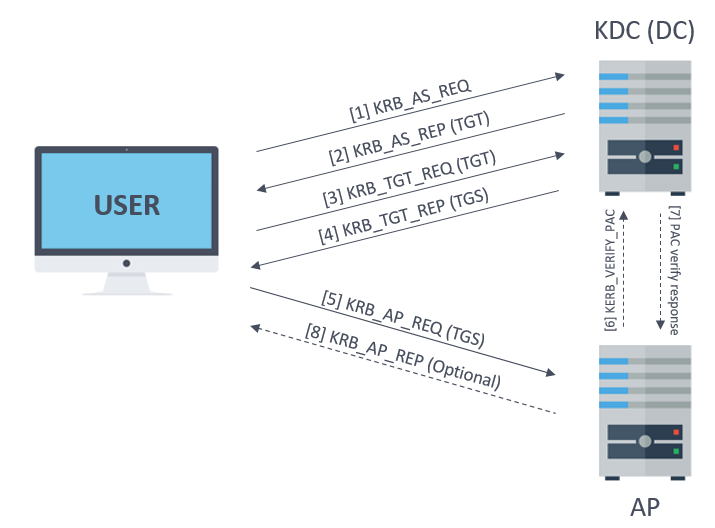
\includegraphics[width=13cm]{img/kerberos_message}
	\caption{Summary of Kerberos messages, obtained from Tarlogic\cite{Tarlogic}.}
	\label{img:tgtTgs}
\end{figure}

It is important to note that Kerberos does not authorize users, but only authenticates them.\\ The authorization is always delegated to each service.

\paragraph{DNS servers}
To communicate inside the internal network, multiple DNS are set up in the domain, so computers can be reached by their name. But these DNS servers do not only answer requests to the internal network, as they are also used as the default DNS servers for all requests to external websites. 

Due to they having this double function, and as explained in \ref{sssec:backProt}, sometimes they can be used to reach the Internet from computers that are not allowed to do web requests.

\subsubsection{Discovery to persist}
\label{sssec:adDisc}
Having information on the users or the configured policies may be crucial when deploying persistence, as many techniques require some previous knowledge of the elements on the domain. Also, some mechanisms do not create or modify anything, but they only need the knowledge of which \textit{objects} (users, computers, etc.) are misconfigured to deploy persistence. 

What is also essential in most persistence techniques is a privileged user, not only on the compromised computer but also in the entire domain. Obtaining the credentials (or the \textit{tickets}) of a user that is \textit{Domain Admin} (or some other role with the same privileges), allows an attacker to create, modify, and remove almost everything domain-related.

\paragraph{Tools to gather AD information}
In order to obtain all the data needed to deploy persistence, or to be able to find both privileged users and computers in the domain, which need to be compromised to acquire their credentials, there are some tools that were created for this type of environment.

These tools use different protocols to gather the data, like LDAP or Kerberos, which are part of the usual traffic within a domain and, therefore, rarely monitored.  

%\pagebreak
\begin{itemize}
\item \textbf{BloodHound - SharpHound}: \underline{BloodHound}\cite{BloodHound} is an application that uses graph theory to reveal the relationships within an Active Directory environment: it associates users to computers, and keeps track of the level of access (ACLs) each user has. 

These relationships, which are often hidden and unintended, can be used to quickly identify highly complex attack paths, and gain a deeper understanding of the existing trust relationships within the domain. 

To better understand what can be achieved with this tool, an example would be that, once a credential is acquired, and therefore it is possible to login into a domain computer, if the compromised user has local admin privileges and additional users are logged too, then their credentials can be retrieved (since they are stored insecurely within memory).\\ If those users have local administrative access on other devices, the attacker would be able to login into other systems and repeat the whole process. 

\underline{SharpHound} is the official data collector for BloodHound\cite{SharpHound}. It uses native Windows API and LDAP functions to collect data from DCs and domain-joined Windows systems.

Once executed, SharpHound automatically determines what domain the current user belongs to, finds a DC for that domain, and starts to collect information depending on the arguments given. 

Some of that collected information is: 
\begin{itemize}
\item Security group memberships
\item Domain trusts 
\item Abusable rights on Active Directory objects
\item Group Policy data
\item SQL admin data
\item Several properties from computer, group, and user objects
\item For each computer, the members of the local administrators, remote desktop, distributed COM, and remote management groups
\item Also for each computer: active sessions, correlated to systems where users are interactively logged on (to know where the credentials are stored)
\end{itemize}

All this information, later exported and displayed on the BloodHound app, can be used to search for the quickest and easiest path to obtain \textit{Domain Admin} privileges, which are needed in most Active Directory persistence techniques.

\item \textbf{Active Directory Explorer}: Microsoft has a set of management tools for Windows environments called "Windows Sysinternals". These programs, which are signed by Microsoft and, consequently, often ignored by antimalware services, can be used to collect information about the computer, the user, and even the domain, among other functionalities.

AD Explorer\cite{ADExplorer} is an advanced Active Directory viewer and editor.  It has multiple uses, such as easily navigating an AD database, viewing object properties and attributes, editing permissions, viewing an object's schema, and executing sophisticated searches. 

Unlike SharpHound, it does not execute loads of queries in a short time (which can be detected by some network monitoring systems), but it is also more difficult to visualize which objects are vulnerable, and it does not collect information about users' sessions in each computer.

\item \textbf{Mimikatz}: This is one of the best tools to gather credential data from Windows systems. Mimikatz\cite{Mimikatz} is an open-source application that allows users to view and save authentication credentials, like plaintext logins and passwords, or Kerberos tickets.  

As it is a very powerful tool, used constantly to escalate privileges and persist in a computer or a network, most security software deletes it as soon as it is detected.\\ However, there are multiple projects based on this program, with the same functionalities but with different names and hashes only to avoid its detection.

It should be noted that almost all of Mimikatz's functionalities \underline{only work with elevated privileges}, which are \textit{Administrator} privileges or even sometimes \texttt{SYSTEM}. 
   
\item \textbf{Other tools to get credentials}: in the next section there is an explanation about some techniques that abuse the Kerberos protocol. To deploy them, multiple tools can be used aside from Mimikatz, like Rubeus or Impacket. 

\underline{Rubeus}\cite{Rubeus} is a tool based on Mimikatz, that has an important characteristic that differentiates it: some of its commands can be run by an unprivileged user, so persistence can be achieved not only with privileged users but also with unprivileged ones.

\underline{Impacket}\cite{Impacket} is a collection of python scripts for working with lots of network protocols, so it has multiple distinct uses. 

\item \textbf{PowerView}: this tool, which is part of the PowerSploit framework\cite{PowerView}, was designed as "a tool to gain network situational awareness on Windows domains". However, its functions can be used to, for example, create users or change their properties, and thus achieve domain persistence.  

\end{itemize}

%\pagebreak
\subsubsection{List of techniques}
\label{sssec:adTec}
As most techniques to deploy persistence in Active Directory need a privileged user to work, it is frequent that, when a domain is compromised, the first tactics to be deployed are \textit{Discovery}\cite{MitreDisc}, \textit{Lateral Movement}\cite{MitreLM}, and \textit{Privilege Escalation}\cite{MitrePE}.

Many of the following techniques use the Active Directory environment (objects, policies, protocols,...) to perform persistences that assure the availability of access to a user that is already an administrator in the domain. But, as stated before, they are only used in combination with other tactics, as they have some requirements. 

Another important note to mention is that most techniques rely on single authentication, something that is currently (and slowly) switching to two-factor authentication. Therefore, some of the listed techniques may become deprecated in the next few years.

But, as AD attacks are typically performed by APTs (explained in section \ref{sssec:apt}), they are frequently not automated but executed manually by adversaries, which makes them better adapted to each environment. 

Finally, and as it is noted on Windows and Linux sections, some of the following techniques have their code in the MITRE ATT\&CK® Matrix\cite{Mitre} written next to their name, for easy classification.

\begin{itemize}
\item \textbf{Accounts: T1136.002 - Creating domain accounts and T1078.002 - Using existing accounts}: with elevated privileges in the domain, new users can be created (which could raise alerts on the security monitoring systems), or credentials of already valid users can be retrieved. 

\vspace{7pt}
\begin{spverbatim}
### The shell command "net" can be used to create new users in the domain ###
> net user /add username password /domain 
\end{spverbatim}
\vspace{7pt}

But the retrieved credentials are not always available in the classical form of "user and password". Instead, getting their network credentials can prove to be useful, since, for example, there is an NTLM hash of the user password (which changes only when the password is changed), or some tickets in Kerberos can be configured to last for years.

\item \textbf{Vulnerable passwords}: although this technique could also be included in section \ref{ssec:persistOthers}, it is particularly prevalent in Active Directory environments, since it is common that administrators set policies about password length, required characters, and expiration date. 

%\pagebreak
When password policies force users to change it each month (as an example), sometimes they use their current month and year to remember it easily, like "October2021". Other times, they use the name of the enterprise plus the month or the year, like "Microsoft102021". These passwords are then \underline{predictable}, and, if leaked or guessed, they could be used as a persistence mechanism because future passwords will be easy to guess too. 

On the other hand, sometimes administrators create users with \underline{never-expiring} passwords (like \textit{service} users), which can lead to the same situation as before. 

For these techniques, even though special privileges might not be required, the compromised users may not have lots of privileges either, as users in \textit{Domain Admin} groups usually have more strict password policies.

\item \textbf{Golden Ticket Attack}: this attack is based on the abuse of Kerberos tickets, as TGTs are essential to obtain TGSs or to authenticate to a network proxy. Consequently, persistence can be achieved if TGTs are stolen (depending on their expiration date, which could be modified to be just minutes or a few years) or if the attacker is able to create their own TGTs. 

To create a TGT, among the necessary, trivial data (username, domain name..), the user \texttt{krbtgt} NTLM Hash is needed. And this hash can only be obtained by having Domain Admin privileges and acquiring it from a Domain Controller.

%...... 
%Encryption keys
%There are several structures handled by Kerberos, as tickets. Many of those structures are encrypted or signed in order to prevent being tampered by third parties. These keys are the following:
%
%KDC or krbtgt key which is derivate from krbtgt account NTLM hash.
%User key which is derivate from user NTLM hash.
%Service key which is derivate from the NTLM hash of service owner, which can be an user or computer account.
%Session key which is negotiated between the user and KDC.
%Service session key to be use between user and service.
%Tickets
%The main structures handled by Kerberos are the tickets. These tickets are delivered to the users in order to be used by them to perform several actions in the Kerberos realm. There are 2 types:
%
%The TGS (Ticket Granting Service) is the ticket which user can use to authenticate against a service. It is encrypted with the service key.
%The TGT (Ticket Granting Ticket) is the ticket presented to the KDC to request for TGSs. It is encrypted with the KDC key.
%
%...... fins aqui lo nou

\pagebreak
\textit{Mimikatz}\cite{Mimikatz} provides multiple methods to obtain the \texttt{krbtgt} hash, like the \textit{DCSync} attack, which tries to impersonate another Domain Controller and request account password information from the targeted Domain Controller. Mimikatz also supports the creation of a Golden Ticket, as can be seen in the following code\cite{GoldenTicket2}:

\vspace{7pt}
\begin{spverbatim}
### Example of commands in Mimikatz to obtain the krbtgt and use it ###
## Obtaining the KRBTGT ##
> lsadump::dcsync /user:krbtgt
## Using that hash to create TGTs impersonating the user 1337 ##
> kerberos::golden /user:username /domain:domain.local /sid:S-1-5-21-3523557010-2506964455-2614950430 /krbtgt:f3bc61e97fb14d18c42bcbf6c3a9055f /id:1337 
\end{spverbatim}
\vspace{7pt}

So the Golden Ticket technique leverages the lack of validation on the Kerberos authentication protocol in order to impersonate a particular user, valid or invalid. This is due to the fact that users that have a TGT in their current session will be considered as trusted for Kerberos, and therefore can try to access any resource in the network.

\item \textbf{Group Policy Objects (GPOs)}: Group Policy Objects contains a set of Group Policies, as explained in \ref{sssec:adBasics}. But, because of their complexity, they are frequently managed by third parties, which usually ends up with lots of users having GPOs with admin rights, unintentionally allowing them to create, modify, and delete Group Policies. And that is an advantage to adversaries, as it makes it easier to find users that can modify GPOs to their benefit. 

In conclusion, even though GPOs were designed to provide simplified management of resources in a domain, they can also be used by an attacker (with privileges)\cite{GPOAttack} to, for example: 
\begin{itemize}
\item push out malware,
\item create/modify scheduled tasks,
\item downgrade credential protections (like changing existing security policies to enable clear-text password extraction),
\item and even add a new administrative local account to all computers.
\end{itemize}
%Some other examples using Mimikatz are:
%\begin{itemize}
%\item Running Invoke-Mimikatz on all Domain Controllers as SYSTEM every week.
%\item Pulling the KRBTGT account and then scheduling a task that runs DCSync on certain computers using forged Kerberos tickets.
%\item Install and re-install malware on every computer in the domain.
%\end{itemize}

Group Policy abuse is related to the technique \textbf{T1037.003 - Boot Initialization Scripts: Network Logon Script}\cite{MitreGPOs}, as it entails the use of network logon scripts to establish persistence, which can be assigned using Group Policy Objects. 
%\item Access Lists ? ACLs

%\item AdminSDHolder

%\pagebreak
\item \textbf{T1556.001 - Modify DC Authentication Process: Skeleton Key}: \textit{Skeleton Key}\cite{SkeletonKey} was a malware used in multiple attacks around 2015, which infected Domain Controllers (DCs) to allow attackers to log as any user in the domain, authorizing them to perform actions in the system, like sending/receiving emails, accessing private files, logging into computers in the domain, etc.

The attack deployed malicious code in a Domain Controller, and that altered the normal Kerberos/NTLM authentication process (it patched the \texttt{lsass.exe} process, which contains user passwords in memory). By doing so, the attackers had the ability to use a new arbitrary password to impersonate any user within the domain, but without the operational risk of changing the actual password of the user (they only changed it in the DC's memory). 

This attack was particularly effective because the DC could continue working and handling authentication requests, and the victim user was still able to use its password; therefore, it only needed minimal changes in the Active Directory structure.

After its disclosure, a very similar feature was added to \textit{Mimikatz}\cite{Mimikatz}, which is the tool used nowadays to execute this technique. 

\begin{spverbatim}
### PowerShell example of the execution of the Skeleton Key technique ###
## First, the Domain Controller needs to be accessed as a user Domain Admin ##
> Invoke-Mimikatz -Command '"privilege::debug" "misc::skeleton"' -ComputerName [name_of_the_DC]

## Then, an attacker can log in as the Administrator user (in this example) in any computer using the password "mimikatz". ##
> Enter-PSSession -ComputerName [name_of_the_computer_to_remotely_access] -Credential [domain_name]\Administrator 
\end{spverbatim}

But, given that the compromised process in this attack (\texttt{lsass.exe}) has been and continues to be used in multiple techniques related to obtaining credentials and elevating privileges, over the years Microsoft has created additional security measures to protect the memory space where this process is hosted (like Protected Process Light (PPL), which enables specially-signed programs to run in a space immune from tampering and termination, even by administrative users). 

For this reason, this technique does not always work, and will depend on the security measures that administrators have implanted on the Domain Controllers.


%DSRM
%users with never expiring passwd
%computers that are DA
% tool: gold finger (FIGHTING GOOOOOOLD)
% ACLs
%- AdminSDHolder
%- SID History
%- Add SPN for Kerberoasting

\end{itemize}

More detailed information about Active Directory, its environment elements and its related attacks and techniques can be found in \cite{AttackingAD}, \cite{DomPersistenceExplained} and \cite{DomPersistenceCommands}.